\documentclass[conference]{IEEEtran}
\IEEEoverridecommandlockouts
% The preceding line is only needed to identify funding in the first footnote. If that is unneeded, please comment it out.
\usepackage{cite}
\usepackage{amsmath,amssymb,amsfonts}
\usepackage{algorithmic}
\usepackage{graphicx}
\usepackage{textcomp}

% jmejia added
\usepackage[utf8]{inputenc}
% \usepackage{algorithm, algpseudocode}
\usepackage{algorithm}
\usepackage{algorithmic}
% jmejia added

\def\BibTeX{{\rm B\kern-.05em{\sc i\kern-.025em b}\kern-.08em
    T\kern-.1667em\lower.7ex\hbox{E}\kern-.125emX}}
\begin{document}

\title{Constraint Handling and Evolutionary Centers Algorithm\\
% {\footnotesize \textsuperscript{*}Note: Sub-titles are not captured in Xplore and
% should not be used}
% \thanks{Identify applicable funding agency here. If none, delete this.}
}

% \institute{%
% Artificial Intelligence Research Center, \\
% University of Veracruz, \\
% Sebasti\'an Camacho 5, Centro \\
% Xalapa, Veracruz, 91000, M\'exico, \\
% jesusmejded@gmail.com; emezura@uv.mx\\
% WWW home pa

\author{\IEEEauthorblockN{1\textsuperscript{st} Jesús-Adolfo Mejía-Dios}
\IEEEauthorblockA{\textit{Artificial Intelligence Research Center} \\
\textit{University of Veracruz}\\
Xalapa, Veracruz, 91000, M\'exico\\
jesusmejded@gmail.com}
\and
\IEEEauthorblockN{2\textsuperscript{nd} Efrén Mezura-Montes}
\IEEEauthorblockA{\textit{Artificial Intelligence Research Center} \\
\textit{University of Veracruz}\\
Xalapa, Veracruz, 91000, M\'exico\\
emezura@uv.mx}
}

\maketitle

\begin{abstract}
Physical phenomena have been the inspiration for proposing different
optimization methods such as electro-search algorithm, central force 
optimization, and charged system search among others. This work presents a new 
optimization algorithm based on some principles from physics and
mechanics, which is called Evolutionary Centers Algorithm (ECA). We utilize 
the center of mass definition for creating new directions for moving the worst 
elements in the population,  based on their objective function values and constraints 
regions, to feasible regions of the search space.  The efficiency of the new 
approach is showed by using the CEC 2017 competition benchmark functions for 
constrained optimization. We present a comparison against a competitive algorithm 
(CAL-SHADE)  in such competition.  The results obtained are promising.
\end{abstract}

\begin{IEEEkeywords}
Constrained optimization, center of mass, evolutionary algorithm, physics-inspired
\end{IEEEkeywords}

\section{Introduction}
Constrained optimization problems are complex to solve due to constraints divide 
the search space into infeasible and feasible search space, highly non-linear 
objective function and large number of variables. Here, we consider the constrained 
optimization problem in the form defined in \cite{cecCop17}:\\

\noindent
Minimize:
\begin{equation}
	f(\vec{x}),\ \vec{x}  \in S \subset \mathbb{R}^D
	\label{eqn:fx}
\end{equation}
%
subject to:
\begin{align*}
	g_i(\vec{x}) &\leq 0,& i =&  1 , \ldots, p \\
	h_j(\vec{x}) &\leq 0,& j =& p+1, \ldots, m
\end{align*}
%
where $S = \prod_{k = 1}^D  [ x_{k,\min},\ x_{k,\max} ]$ i.e. 
$x_k \in [ x_{k,\min},\ x_{k,\max} ]$ for $k = 1,2,\ldots,D$.  The problem is 
subject to $p$ inequality constraints and $m - p$ equality constraints. If 
$\vec{x}$ satisfies $g_i( \vec{x} ) \leq 0$, for $i = 1, \ldots, p$ and 
$|h_j(\vec{x})| \leq \varepsilon$, for $j = p+1, \ldots, m$ with 
$\varepsilon > 0$ a small value; then $\vec{x}$ is regarded feasible.\\


The rest of the paper is organized as follows. A brief review of population-based 
algorithms for constrained optimization problems is presented in Section \ref{sec:related_work}. 
Section \ref{sec:eca} describes the proposal of new meta-heuristic for the solution 
of constrained optimization problem and the constrained handling. Specification of 
experiments and control parameter setting are given in Section \ref{sec:experiments}. 
Experimental results including and a comparison against a competitive algorithm 
are presented in Section \ref{sec:results}. Conclusions and future work are made 
in Section \ref{sec:conclusions} and \ref{sec:future_work} respectively.


\section{Related Work} % (fold)
\label{sec:related_work}

Population based algorithm can be classified into three main classes:
evolutionary, physics-based, and swarm intelligence algorithms.
Some of the EAs are Genetic Algorithm \cite{melanie96}, Differential Evolution 
(DE) \cite{ed1995}, Evolutionary Programing (EP), Evolution Strategy (ES) and 
Genetic Programming (GP) \cite{back,spall03}.
%
The most popular EA algorithm for real-parametric optimization is Differential 
Evolution (DE). DE was introduced by Storn and Price \cite{ed1995}  for global 
optimization over continuous spaces.\\
%

The second main branch of meta-heuristics are physical metaphors inspired algorithms
Some of the most popular algorithms are Gravitational  Search Algorithm (GSA) 
\cite{rashedi2009gsa}, Gravitational Local Search (GLSA) \cite{glsa}, Big-Bang 
Big-Crunch (BBBC) \cite{erol2006new}, Charged System Search (CSS) \cite{kaveh2010novel}, 
Central Force Optimization (CFO) \cite{cfo2007}, Black Hole (BH) \cite{hatamlou2013black} 
algorithm, Ray Optimization (RO) algorithm \cite{kaveh2012new}. Here some recent 
surveys on this topic \cite{fisicaSurvey,biswas2013physics,xie2011convergence,DBLP:journals/corr/FisterYFBF13}. 
This kind of algorithms emulate physical systems, for example, in CFO each solution 
is a body and they move and interact through the space using gravitational force.\\
% 

Finally, the swarms intelligence (SI) methods simulates a social behavior of 
swarms. Here, each search agents navigate using the simulated collective and 
social intelligence  of creatures. The most popular SI techniques are particle 
swarm optimization (PSO)  \cite{pso1995}, and the artificial bee colony (ABC) 
\cite{abc2005}. The PSO algorithm  is inspired from the social behavior of birds 
flocking.\\

In this work, we employ CFO, PSO and ABC equation for generating new solutions. 
The relationship among those algorithms is their mathematical formulation for 
generating solutions through an iterative process:
%
\begin{equation}
	\vec{x}_{i + 1} = \vec{x}_{i} + \vec{v}_{i + 1}
	\label{eqn:xxv}
\end{equation}
%
where each algorithm updates $\vec{v}_{i+1} $ as follows:
\begin{itemize}
	\item CFO: $$
		\vec{v}_{i + 1} = \omega \vec{v}_{i} + {\lambda \vec{F}_{i}} / {m_i},
		$$
		where $\vec{v}_{i}$ is the current solution, $\lambda$ is a uniformly 
		distributed random variable in [0, 1], $\omega$ 
		is user-defined weight $0 < \omega < 1$, $m_i,\; F_i$ are mass and force 
		functions, respectively, both defined by the authors.
	\item PSO:
		$$
			\vec{v}_{i + 1} = \omega \vec{v}_{i} +  
					c_1 r_{1, i} ( \vec{x}_{pbest, i} - \vec{x}_i ) + 
					c_2 r_{2, i} ( \vec{x}_{gbest, i} - \vec{x}_i ),
		$$
		where $\omega$ is a inertia weight used for balancing the global search 
		and local search, $\vec{x}_{pbest, i}$ and $\vec{x}_{gbest, i}$ are the 
		best position reached by solution $i$ so far and the best solution in the 
		population, respectively; $c_1$ and $c_2$ are two positive constants, 
		$r_{1, i},\; r_{2, i}$  are random numbers with uniform distribution in 
		the range [0, 1].
	%%%%%%%%%%%%%%%%%%%%%%%%%%%%%%%%%%%%
	\item ABC:
		$$
			\vec{v}_{i + 1} = \phi_i (\vec{x}_i - \vec{x}_{r}),
		$$
	where $\vec{x}_i$ is the current solution, $\vec{x}_r$ is a randomly chosen 
	solution, $\phi_i$ is a randomly produced number with uniform distribution 
	in the interval $[-1,\;1]$.
	%%%%%%%%%%%%%%%%%%%%%%%%%%%%%%%%%%%%
\end{itemize}
%
%
In the three previous cases, the $\vec{v}$ value  depends of the population 
distribution at current generation $i$.

The following Section \ref{sec:eca} describes our algorithm and how it 
relates to what has been  described above. 

% section related_work (end)

\section{Evolutionary Centers Algorithm} % (fold)
\label{sec:eca}

In this section, constraint handling (CH) and evolutionary centers algorithm (ECA) 
is detailed. First, ECA is detailed and consequently CH take place for CH-ECA 
implementation.\\

Our approach is based on the center of mass definition and is utilized for creating 
new directions for moving the worst  elements in the population, based on their 
objective function values and constraint violations, to feasible regions of the 
search space.

%
%
\subsection{Motivation} % (fold)
The center of mass is a geometric property of any body. Intuitively, it is the 
average location of the weight of an object. We can completely describe the motion 
of any object through space in terms of the translation of the center of mass of 
the object from one place to another. This is the motivation for using the center 
of mass concept, we translate the population to places where the mass of the entire 
population is maximum.
% 

In mathematical terms, the center of mass is the unique point $\vec{c}$ at the 
center of a distribution of mass $U = \{\vec{u}_1,\; \vec{u}_2 , \ldots , \vec{u}_K \}$ 
in a space that has the property that the weighted sum of position vectors 
relative to this point  is zero \cite{kleppner73,serway}. That is:
%
%
\begin{equation}
	\sum_{i = 1}^K m(\vec{u}_i) (\vec{u}_i - \vec{c}) = 0, \text{ implies } 
	%%%%%%%%%%%%%%%%%%%%%
	\vec{c} = \dfrac{1}{M} \sum_{i = 1}^K  m(\vec{u}_i)  \vec{u}_i,
	\label{eq:masscenter}
\end{equation}
%
%
where $m(\vec{u}_i)$ is the mass of $\vec{u}_i$ and  $M$ is the sum of the 
masses of vectors in $U$. Here, $m$ is a non-negative function. Similar as in 
Statistics, the center of mass is the mean location of a distribution 
of mass in space.\\


In this work, the objective function of the optimization problem represents 
the mass of each solution in the population,  i.e., we set $f(\vec{x}) = m(\vec{x})$ 
for all $\mathbb{R}^D$.  Without loss of generality, we assume that we want to 
maximize  the non-negative function $f$.




\subsection{Algorithm Description} % (fold)
\label{sub:algorithm_description}

For each solution $\vec{x}_i $ in the population $P = \{ \vec{x}_1, \vec{x}_2, \ldots, \vec{x}_{N} \} $ 
of $N$  solutions, we select a subset $U \subset P $ with $K$ solutions; then, 
from $U$ we obtain the center of mass $\vec{c}$. After that, based on 
a randomly chosen solution $\vec{u}_r \in U$,  
and the already generated center of mass $\vec{c}$, we generate a direction 
to locate a new solution $ \vec{h}_i$. We suggest using the following strategy:

\begin{equation}
	\vec{y}_i = \vec{x}_i + \eta _{i} ( \vec{c}_i - \vec{u}_{r} ),
	\label{eqn:vcu}
\end{equation}
%
where 
%
\begin{equation}
	\vec{c}_i = \dfrac{1} {W} \sum_{u \in U} f(\vec{u}) \cdot \vec{u} , 
			\hspace{0.5cm} 
			W = \sum_{ \vec{u} \in U} f(\vec{u}).
	\label{eqn:center}
\end{equation}

If $f$ is a positive constant function, then the center of mass of $U$ is the 
geometric center of  $U$. That is, assume that $f(\vec{x}) = \alpha$ for every 
$\vec{x} \in \mathbb{R}^D$,  with $\alpha$ a positive constant. The 
center of mass is:
%
%
\begin{equation}
	\vec{c}_i = \dfrac{1} {K \alpha} \sum_{ \vec{u} \in U} \alpha \cdot \vec{u} %
			  =  \dfrac{1} {K } \sum_{\vec{u} \in U} \vec{u}.
	\label{eqn:center-geometric}
\end{equation}
%
%
Thus, for a constant mass function, we have the center of mass converging 
to the geometric center. In real world problems, functions can be flat 
in some regions, then this algorithm may find some difficulties  when 
dealing with such issue.

\begin{figure}[!ht]
	\centering
	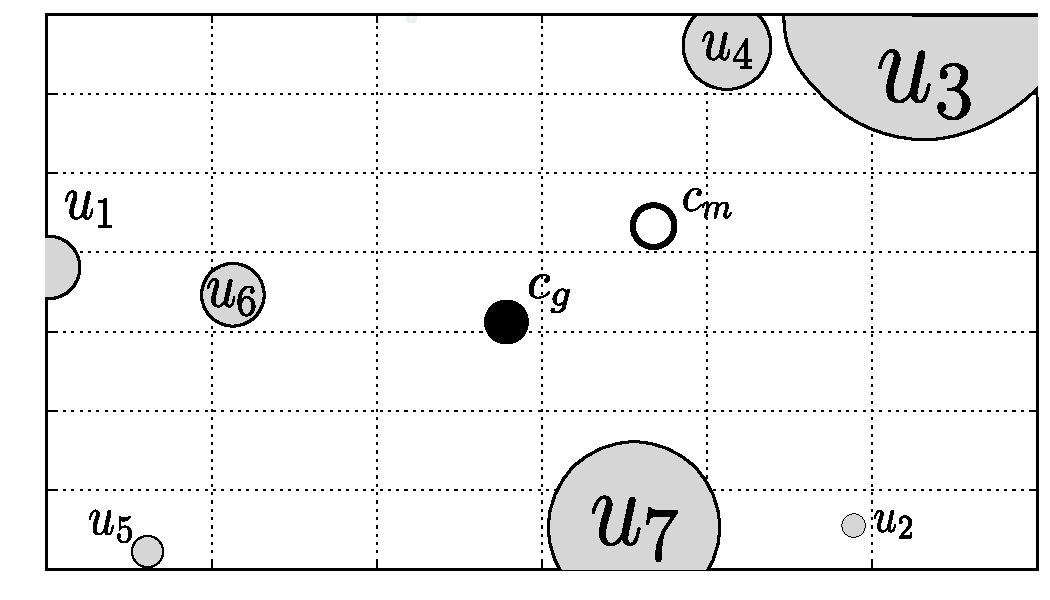
\includegraphics[width=7cm]{img/masses.pdf}
	\caption{$c_m$ is center of mass, $c_g$ is geometric center of black points. %
	Gray point radius is its mass. Note the bias given by the weighted sum.}
	\label{fig:masses}       % Give a unique label
\end{figure}
%
%
The bias is given by Equation (\ref{eqn:center}) because for a solution 
with the highest mass, the position of the center of mass is nearest to 
its position, see Figure \ref{fig:masses}.
%

\subsection{Constraint Handling} % (fold)
\label{sec:constraint_handling}

Initialization with feasible solutions is very time consuming process and in some 
cases it is impossible to produce a feasible solution randomly \cite{castillofoundations}, 
CH-ECA does not consider the initial population to be feasible. Now, consider the 
following rules for constraint handling. For a constrained optimization problem, 
we select $\vec{y}$ instead $\vec{x}$ if

\begin{equation}
	\begin{cases}
	\overline{\nu}( \vec{y} ) < \overline{\nu}( \vec{x} )  \text{ or}\\
	% 
	\overline{\nu}( \vec{y} ) = \overline{\nu}( \vec{x} ) \text{ and } f(\vec{y}) > f(\vec{x})
		% 
	\end{cases}
	\label{eqn:rules}
\end{equation}
where $\overline{\nu}$ is the mean value of all constraints’ violations defined as:

\begin{equation}
	\overline{\nu}( \vec{x} ) = \dfrac{1}{m} \left[ \sum_{i=1}^q G_i(\vec{x}) + \sum_{j=q+1}^m H_i(\vec{x}) \right],
	\label{eqn:nu}
\end{equation}
%
with 
\begin{eqnarray}
	G_i(\vec{x}) &=&
	\begin{cases}
		g_i(\vec{x})   & g_i(\vec{x}) > 0,  \\
		    0          & g_i(\vec{x}) \leq 0,
	\end{cases}
	\\
	%
	H_i(\vec{x}) &=&
	\begin{cases}
		|h_i(\vec{x})|   & |h_i(\vec{x})| - \varepsilon  > 0,  \\
		    0            & |h_j(\vec{x})| - \varepsilon \leq 0
	\end{cases}
	.
	%
\end{eqnarray}
%
Note that, $G_i(\vec{x})$ and $H_i(\vec{x})$ are zero when the solution is feasible. 
Also, they are non-negative functions. Here, according to \cite{cecCop17}, we set 
tolerance $\varepsilon = 0.0001$ and $g_i(\vec{x}) \leq 0,\ h_j(\vec{x}) = 0$ are 
$m$ constraints.\\

Structure of the algorithm already directs the solutions to feasible region in 
running process due to the rules in Equation  \ref{eqn:rules} employed.


\subsection{Population Replacement} % (fold)

Let $P$ and $A$  be  non-empty sets of individuals. Random elements in $P$ are 
replaced with elements in $A$ if they are not better than elements in $A$.

\begin{figure}[!ht]
	\centering
	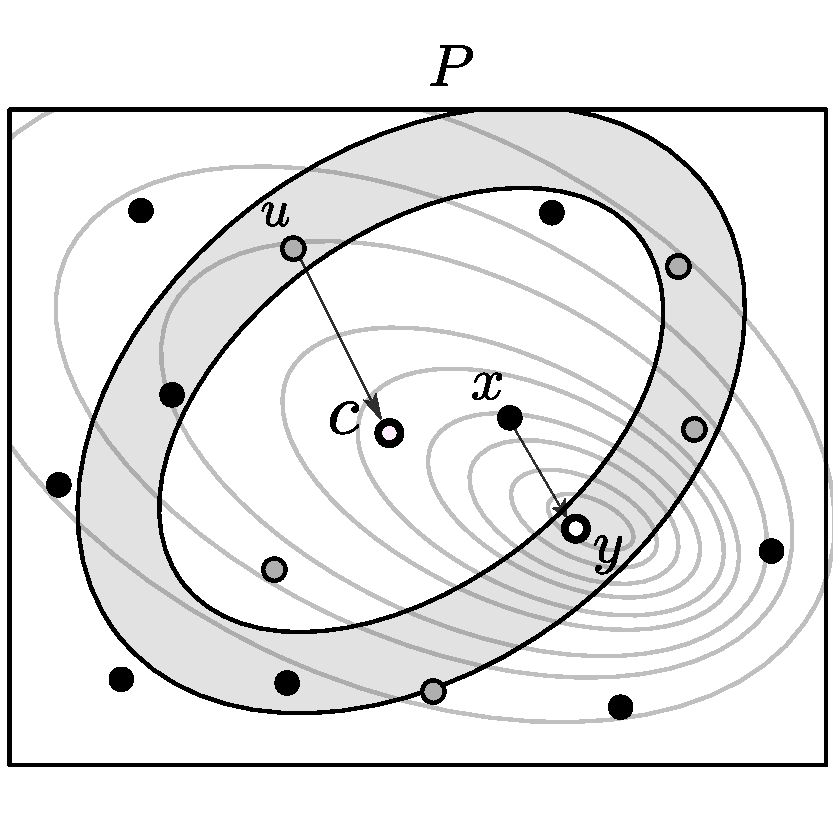
\includegraphics[width=5cm]{img/ecaG.pdf}
	\caption{Schematic diagram representing a generation of CH-ECA. Gray points % 
	represent elements in $U$. Gray area is representing the feasible region.}
	\label{fig:ecag}       % Give a unique label
\end{figure}

Note that our approach (see Algorithm \ref{alg:ch.eca}) has only two parameters: 
the number of neighbors $K$ and  the stepsize $\eta_{\max}$.  For large $K$ values, 
CH-ECA could converge  faster, we suggest $K = 7$, a value obtained experimentally. 
Figure \ref{fig:ecag} shows a representation of CH-ECA solution update. 

\begin{algorithm}[!ht]
	\caption{CH-ECA Algorithm}
	\label{alg:ch.eca}
	\begin{algorithmic}[1]
 		\renewcommand{\algorithmicrequire}{\textbf{Input:}}
 		\renewcommand{\algorithmicensure}{\textbf{Output:}}
		\REQUIRE {$K = 7, \; \eta_{\max} = 2$}
		%\State poplulation size = 20 $\times$ dimension
		\STATE $N \gets 2K * D$
		\STATE Generate and evaluate start population $P$ with $N$ elements
		\STATE { Evaluate $g_i$ and $h_j$ constraints}
		\WHILE{the end criterion is not achieved}
			\STATE $A = \emptyset$
			\FOR {each $\vec{x}$ in $P$}
				\STATE Generate $U \subset P$ such that  card$(U) = K$
				\STATE Calculate $\vec{c}$ using $U$ with (\ref{eqn:center})
				\STATE $\eta \gets \text{rand}(0,\; \eta_{\max}) $ 
				\STATE $\vec{y} \gets \vec{x} + \eta  * (\vec{c} - \vec{u}) $ %
						where $ \vec{u} \in U $ random
				
				\IF{ $\vec{y}$ or $\vec{x}$ using rules \ref{eqn:rules}}
					\STATE Append $\vec{y} $ in $A$
				\ENDIF
			\ENDFOR
			\STATE {   $P \gets $ best elements in $P \cup A$}
			% \STATE 
		\ENDWHILE
		\RETURN { best solution} in $P$
		% \EndProcedure
	\end{algorithmic}
\end{algorithm}

% section constraint_handling (end)

\section{Experiments} % (fold)
\label{sec:experiments}

In order to evaluate the performance of the CH-ECA, we used a set of
28 benchmark problems can be found in \cite{cecCop17}. This set includes both 
forms of objective function such as separable and non-separable.\\

According to problem set \cite{cecCop17}, maximum function evaluations (MAXFES) 
was set at $20000 \times D$ and 25 independent runs of the proposed algorithm 
were recorded on 28 test problem functions for $D = 10, 30, 50$ and 100, with 
the same CH-ECA parameters for all experiments:

\begin{itemize}
	\item Inputs: $K = 7$, $\eta_{\max} = 2$. 
	\item Population size: $N = 2K * D$.
	\item Stop Condition: when MAXFES is reached.
	\item $\eta$ in step 9 in Algorithm \ref{alg:ch.eca} is a uniform random 
		  number between in $(0,\ \eta_{\max} ]$.
\end{itemize}

This benchmark contains a wide variety of objective and constraint functions. The 
mathematical formulas and properties of these functions are described explicitly 
but they are treated as a black box problem \cite{jones1998efficient}.

% section experiments (end)

\section{Results} % (fold)
\label{sec:results}

Results show best, worst, mean, and standard deviation values of objective 
function  and SR which is the feasibility rate defined as 
\textit{(\# of feasible runs) / Total runs},  where a feasible run is a run 
during which at least one feasible solution is found in MAXFES.\\
% 

Experimental results obtained by CH-ECA are reported in Tables \ref{tab:d10}, \ref{tab:d30}, 
\ref{tab:d50} and \ref{tab:d100} for dimension 10, 30, 50 and 100 respectively. 
It is worth noting that CH-ECA obtained results on feasible regions (feasible 
ratio equal 100\%) while reporting low standard deviation values. Therefore, CH-ECA 
behavior can be considered as robust and suitable to deal with different type of 
search spaces and feasible regions. This was observed in low dimensions. \\
% 

Furthermore, we compared CH-ECA against a  competitive algorithm in 
the CEC 2017 competition on constrained real-parameter single-objective optimization 
(CAL-SHADE) \cite{zamuda2017adaptive}, which is an adaptive algorithm based on 
differential evolution. The comparison based on 25 independent runs by each algorithm 
is presented in Tables \ref{tab:d10c}, \ref{tab:d30c}, \ref{tab:d50c} and 
\ref{tab:d100c} for dimension 10, 30, 50 and 100 respectively. In such Tables last 
column contain a ``$\approx$'', ``--'' or ``+'' symbol. ``+'' means that CH-ECA 
outperformed CAL-SHADE in the function in the corresponding row, ``-'' means that 
CAL-SHADE outperformed ECA, and  ``$\approx$'' means that no difference was 
observed between algorithms. Here, ``algorithm $\mathcal{A}_1$ outperforms algorithm 
$\mathcal{A}_2$'' means SR$_{\mathcal{A}_1} > $ SR$_{\mathcal{A}_2}$ or 
(SR$_{\mathcal{A}_1} = $ SR$_{\mathcal{A}_2}) \wedge ($ Mean$_{A_1} < $ Mean$_{A_2}$). 
This is a simplified ranking method based on \cite{cecCop17}. \\

As we can see in Table \ref{tab:d10c}, CH-ECA was able to outperform CAL-SHADE in 
eighteen test functions, it reached similar results in two test problems, and 
finally CH-ECA was outperformed by CAL-SHADE in eight functions. CH-ECA was then 
competitive in twenty test problems. %
%
Table \ref{tab:d30c} shows that our approach was able to outperform CAL-SHADE in 
twelve test functions and CH-ECA was outperformed by CAL-SHADE in sixteen functions.
%
In Table \ref{tab:d50c} and \ref{tab:d100c} show a poor performance because of 
highly dimensionality. Those results are summarized in Table \ref{tab:summary}.

\begin{table}[!ht]
	\caption{Performance Summary.}
	\label{tab:summary}
	% 
	\centering
	\begin{tabular}{c|ccc}
		$D$ & ``+'' &  -- & ``$\approx$'' \\ \hline
		10  & 18    &  6  & 4  \\ \
		30  & 12    &  14 & 2  \\ \
		50  & 8     &  16 & 4 \\ \
	   100  & 5     &  13 & 10  \\ \
	\end{tabular}
\end{table}


Finally, CH-ECA is more simple to implement than CAL-SHADE and requires less 
mechanisms to operate.

% \clearpage
\section{Conclusions} % (fold)
\label{sec:conclusions}

A new meta-heuristic optimization algorithm, denoted as Constraint Handling and 
Evolutionary Centers  Algorithm, inspired by the center of mass of a system of 
particles was proposed with constraint handling mechanism that prioritizes the 
feasible solutions before infeasible. The results showed the capability of CH-ECA 
to consistently reach feasible regions  in different types of search spaces. CH-ECA also provided 
a competitive, but still not better, performance against a competitive algorithm 
in such  competition on constrained real-parameter single-objective optimization. 
CH-ECA  is a simple algorithm which requires the fine-tuning of just two parameters 
($K$ and $\eta_{\max}$),  besides the population size.

% section conclusions (end)

\section{Future Work} % (fold)
\label{sec:future_work}

The performance of CH-ECA can be also tested for real-world problems existing in 
the literature and compared with that of other algorithms. Also, the effect of 
constraint handling methods on the performance of the CH-ECA is part the future 
work derived from this current research. 
% section future_work (end)


\bibliographystyle{IEEEtran}
\bibliography{IEEEabrv,references}

\clearpage
\begin{table}[!ht]
	\caption{Function values achieved when the stopping condition is reached for $10D$ problems.}
	% 
	\centering
	\begin{tabular}{|c|c|c|c|c|c|c|}
	\hline
     & Best & Worst & Mean & Std. & SR \\ \hline \hline
C01 & 0.000E+00 & 0.000E+00 & 0.000E+00 & 0.000E+00 &  100 \\ 
C02 & 0.000E+00 & 0.000E+00 & 0.000E+00 & 0.000E+00 &  100 \\ 
C03 & 0.000E+00 & 0.000E+00 & 0.000E+00 & 0.000E+00 &  100 \\ 
C04 & 1.691E+01 & 1.691E+01 & 2.894E+01 & 6.935E+00 &  100 \\ 
C05 & 0.000E+00 & 0.000E+00 & 0.000E+00 & 0.000E+00 &  100 \\ 
C06 & 6.965E+00 & 6.965E+00 & 1.421E+01 & 5.669E+00 &  100 \\ 
C07 &  -- &  -- &  -- &  -- &    0 \\ 
C08 &  -- &  -- &  -- &  -- &    0 \\ 
C09 & 2.851E+00 & 2.851E+00 & 5.916E+00 & 2.431E+00 &   32 \\ 
C10 &  -- &  -- &  -- &  -- &    0 \\ 
C11 &  -- &  -- &  -- &  -- &    0 \\ 
C12 & 0.000E+00 & 0.000E+00 & 8.988E--01 & 1.556E+00 &  100 \\ 
C13 & 0.000E+00 & 0.000E+00 & 4.784E--01 & 1.322E+00 &  100 \\ 
C14 & 0.000E+00 & 0.000E+00 & 0.000E+00 & 0.000E+00 &  100 \\ 
C15 & -9.999E+00 & -9.999E+00 & -5.381E+00 & 2.641E+00 &  100 \\ 
C16 & 6.432E+09 & 6.432E+09 & 6.593E+09 & 1.050E+08 &   80 \\ 
C17 & 0.000E+00 & 0.000E+00 & 0.000E+00 & 0.000E+00 &  100 \\ 
C18 & 0.000E+00 & 0.000E+00 & 7.147E+00 & 1.598E+01 &   20 \\ 
C19 &  -- &  -- &  -- &  -- &    0 \\ 
C20 & 2.715E+00 & 2.715E+00 & 2.888E+00 & 6.640E--02 &  100 \\ 
C21 & 0.000E+00 & 0.000E+00 & 8.175E--01 & 1.380E+00 &  100 \\ 
C22 & 0.000E+00 & 0.000E+00 & 6.379E--01 & 1.492E+00 &  100 \\ 
C23 & 0.000E+00 & 0.000E+00 & 0.000E+00 & 0.000E+00 &  100 \\ 
C24 & -1.000E+01 & -1.000E+01 & -6.833E+00 & 3.087E+00 &  100 \\ 
C25 & 5.906E+08 & 5.906E+08 & 5.906E+08 & 0.000E+00 &  100 \\ 
C26 & 0.000E+00 & 0.000E+00 & 0.000E+00 & 0.000E+00 &  100 \\ 
C27 & 0.000E+00 & 0.000E+00 & 5.786E+00 & 9.881E+00 &   28 \\ 
C28 &  -- &  -- &  -- &  -- &    0 \\ 
\hline
	\end{tabular}
	\label{tab:d10}
\end{table}
% 
% 
% 
\begin{table}[!ht]
	\caption{Function values achieved when the stopping condition is reached for $30D$ problems.}
	% 
	\centering
	%
	\begin{tabular}{|c|c|c|c|c|c|c|}
	\hline
     & Best & Worst & Mean & Std. & SR \\ \hline \hline
C01 & 3.204E--08 & 3.204E--08 & 4.167E--06 & 1.090E--05 &  100 \\ 
C02 & 0.000E+00 & 0.000E+00 & 2.285E--05 & 1.024E--04 &  100 \\ 
C03 & 1.889E--07 & 1.889E--07 & 1.871E--05 & 3.904E--05 &  100 \\ 
C04 & 1.086E+02 & 1.086E+02 & 1.543E+02 & 4.942E+01 &  100 \\ 
C05 & 1.219E+01 & 1.219E+01 & 2.363E+01 & 1.265E+01 &  100 \\ 
C06 & 9.400E+01 & 9.400E+01 & 1.532E+02 & 4.291E+01 &  100 \\ 
C07 &  -- &  -- &  -- &  -- &    0 \\ 
C08 &  -- &  -- &  -- &  -- &    0 \\ 
C09 & 7.430E+00 & 7.430E+00 & 1.108E+01 & 4.812E+00 &   20 \\ 
C10 &  -- &  -- &  -- &  -- &    0 \\ 
C11 &  -- &  -- &  -- &  -- &    0 \\ 
C12 & 5.450E+00 & 5.450E+00 & 1.124E+01 & 7.533E+00 &  100 \\ 
C13 & 1.284E+04 & 1.284E+04 & 3.496E+04 & 1.713E+04 &   48 \\ 
C14 & 7.419E--05 & 7.419E--05 & 6.191E--01 & 5.670E--01 &  100 \\ 
C15 & -3.927E+00 & -3.927E+00 & 8.496E--01 & 3.285E+00 &  100 \\ 
C16 & 3.823E+10 & 3.823E+10 & 3.894E+10 & 4.687E+08 &  100 \\ 
C17 & 7.607E--07 & 7.607E--07 & 1.301E--01 & 1.705E--01 &  100 \\ 
C18 & 2.025E+01 & 2.025E+01 & 3.923E+01 & 2.685E+01 &    8 \\ 
C19 &  -- &  -- &  -- &  -- &    0 \\ 
C20 & 1.133E+01 & 1.133E+01 & 1.159E+01 & 1.475E--01 &  100 \\ 
C21 & 6.404E+00 & 6.404E+00 & 1.353E+01 & 1.029E+01 &  100 \\ 
C22 & 2.616E+04 & 2.616E+04 & 5.120E+04 & 2.044E+04 &   24 \\ 
C23 & 2.141E--04 & 2.141E--04 & 4.647E--01 & 5.912E--01 &  100 \\ 
C24 & -3.927E+00 & -3.927E+00 & 2.105E+00 & 2.856E+00 &  100 \\ 
C25 &  -- &  -- &  -- &  -- &    0 \\ 
C26 & 1.156E--06 & 1.156E--06 & 1.073E--01 & 1.746E--01 &  100 \\ 
C27 & 2.025E+01 & 2.025E+01 & 3.216E+01 & 1.406E+01 &   16 \\ 
C28 &  -- &  -- &  -- &  -- &    0 \\ 
\hline
	\end{tabular}
	\label{tab:d30}
\end{table}
% 
% 
% 
\begin{table}[!ht]
	\caption{Function values achieved when the stopping condition is reached for $50D$ problems.}
	% 
	\centering
	%
	\begin{tabular}{|c|c|c|c|c|c|c|}
	\hline
     & Best & Worst & Mean & Std. & SR \\ \hline \hline
C01 & 4.914E+01 & 4.914E+01 & 2.660E+02 & 1.941E+02 &  100 \\ 
C02 & 2.645E+01 & 2.645E+01 & 2.080E+02 & 1.326E+02 &  100 \\ 
C03 & 1.827E+02 & 1.827E+02 & 7.052E+02 & 3.771E+02 &  100 \\ 
C04 & 2.008E+02 & 2.008E+02 & 2.990E+02 & 4.828E+01 &  100 \\ 
C05 & 8.247E+01 & 8.247E+01 & 1.912E+02 & 7.258E+01 &  100 \\ 
C06 & 2.817E+02 & 2.817E+02 & 4.674E+02 & 1.096E+02 &  100 \\ 
C07 &  -- &  -- &  -- &  -- &    0 \\ 
C08 &  -- &  -- &  -- &  -- &    0 \\ 
C09 & 6.711E+00 & 6.711E+00 & 1.081E+01 & 2.946E+00 &   36 \\ 
C10 &  -- &  -- &  -- &  -- &    0 \\ 
C11 &  -- &  -- &  -- &  -- &    0 \\ 
C12 &  -- &  -- &  -- &  -- &    0 \\ 
C13 &  -- &  -- &  -- &  -- &    0 \\ 
C14 &  -- &  -- &  -- &  -- &    0 \\ 
C15 & 2.356E+00 & 2.356E+00 & 6.629E+00 & 2.991E+00 &  100 \\ 
C16 & 7.558E+10 & 7.558E+10 & 7.641E+10 & 6.619E+08 &  100 \\ 
C17 & 7.229E--01 & 7.229E--01 & 9.250E--01 & 1.002E--01 &   76 \\ 
C18 &  -- &  -- &  -- &  -- &    0 \\ 
C19 &  -- &  -- &  -- &  -- &    0 \\ 
C20 & 2.036E+01 & 2.036E+01 & 2.067E+01 & 1.931E--01 &  100 \\ 
C21 &  -- &  -- &  -- &  -- &    0 \\ 
C22 &  -- &  -- &  -- &  -- &    0 \\ 
C23 &  -- &  -- &  -- &  -- &    0 \\ 
C24 & 2.356E+00 & 2.356E+00 & 9.142E+00 & 3.591E+00 &  100 \\ 
C25 & 1.925E+09 & 1.925E+09 & 1.925E+09 & 0.000E+00 &  100 \\ 
C26 & 9.131E--01 & 9.131E--01 & 9.807E--01 & 4.522E--02 &   16 \\ 
C27 &  -- &  -- &  -- &  -- &    0 \\ 
C28 &  -- &  -- &  -- &  -- &    0 \\ 
\hline
	\end{tabular}
	\label{tab:d50}
\end{table}
% 
% 
% 
\begin{table}[!ht]
	\caption{Function values achieved when the stopping condition is reached for $100D$ problems.}
	% 
	\centering
	%
	\begin{tabular}{|c|c|c|c|c|c|c|}
	\hline
     & Best & Worst & Mean & Std. & SR \\ \hline \hline
C01 & 4.989E+03 & 4.989E+03 & 8.793E+03 & 2.057E+03 &  100 \\ 
C02 & 2.969E+03 & 2.969E+03 & 4.915E+03 & 1.300E+03 &  100 \\ 
C03 & 5.570E+03 & 5.570E+03 & 9.405E+03 & 1.963E+03 &  100 \\ 
C04 & 6.627E+02 & 6.627E+02 & 8.400E+02 & 1.464E+02 &  100 \\ 
C05 & 3.068E+03 & 3.068E+03 & 6.806E+03 & 2.636E+03 &  100 \\ 
C06 & 1.147E+03 & 1.147E+03 & 1.494E+03 & 1.980E+02 &  100 \\ 
C07 &  -- &  -- &  -- &  -- &    0 \\ 
C08 &  -- &  -- &  -- &  -- &    0 \\ 
C09 &  -- &  -- &  -- &  -- &    0 \\ 
C10 &  -- &  -- &  -- &  -- &    0 \\ 
C11 &  -- &  -- &  -- &  -- &    0 \\ 
C12 &  -- &  -- &  -- &  -- &    0 \\ 
C13 &  -- &  -- &  -- &  -- &    0 \\ 
C14 &  -- &  -- &  -- &  -- &    0 \\ 
C15 & 8.639E+00 & 8.639E+00 & 1.442E+01 & 1.740E+00 &  100 \\ 
C16 & 9.061E+10 & 9.061E+10 & 9.184E+10 & 6.868E+08 &  100 \\ 
C17 &  -- &  -- &  -- &  -- &    0 \\ 
C18 &  -- &  -- &  -- &  -- &    0 \\ 
C19 &  -- &  -- &  -- &  -- &    0 \\ 
C20 & 4.384E+01 & 4.384E+01 & 4.418E+01 & 1.906E--01 &  100 \\ 
C21 &  -- &  -- &  -- &  -- &    0 \\ 
C22 &  -- &  -- &  -- &  -- &    0 \\ 
C23 &  -- &  -- &  -- &  -- &    0 \\ 
C24 & 1.492E+01 & 1.492E+01 & 2.225E+01 & 4.730E+00 &   24 \\ 
C25 &  -- &  -- &  -- &  -- &    0 \\ 
C26 &  -- &  -- &  -- &  -- &    0 \\ 
C27 &  -- &  -- &  -- &  -- &    0 \\ 
C28 &  -- &  -- &  -- &  -- &    0 \\ 
\hline
	\end{tabular}
	\label{tab:d100}
\end{table}

% 
% 
% 
\begin{table}[!ht]
	\caption{Function values achieved when the stopping condition is reached for $10D$ problems.}
	% 
	\centering
	%
	\begin{tabular}{|c|r|r|c|c|c|}
	 \hline
	 &\multicolumn{2}{|c|}{Mean} & \multicolumn{2}{|c|}{SR} & \\
	\cline{2-5}
	    & CH-ECA & CAL-SHADE & CH-ECA & CAL-SHADE & \\ \hline
C01 & 0.000E+00 & 0.000E+00 &  100 &  100 & $\approx$ \\ 
C02 & 0.000E+00 & 0.000E+00 &  100 &  100 & $\approx$ \\ 
C03 & 0.000E+00 & 1.100E+05 &  100 &   44 & + \\ 
C04 & 2.894E+01 & 3.874E+01 &  100 &  100 & + \\ 
C05 & 0.000E+00 & 9.568E--01 &  100 &  100 & + \\ 
C06 & 1.421E+01 & 5.496E+02 &  100 &   96 & + \\ 
C07 &  -- & -4.874E+01 &    0 &   68 & -- \\ 
C08 &  -- & -1.348E--03 &    0 &  100 & -- \\ 
C09 & 5.916E+00 & 1.255E--01 &   32 &  100 & -- \\ 
C10 &  -- & -5.100E--04 &    0 &  100 & -- \\ 
C11 &  -- & -1.563E--01 &    0 &  100 & -- \\ 
C12 & 8.988E--01 & 3.988E+00 &  100 &  100 & + \\ 
C13 & 4.784E--01 & 1.116E+00 &  100 &  100 & + \\ 
C14 & 0.000E+00 & 2.641E+00 &  100 &  100 & + \\ 
C15 & -5.381E+00 & 1.625E+01 &  100 &   68 & + \\ 
C16 & 6.593E+09 & 6.542E+01 &   80 &   60 & + \\ 
C17 & 0.000E+00 &  -- &  100 &    0 & + \\ 
C18 & 7.147E+00 &  -- &   20 &    0 & + \\ 
C19 &  -- &  -- &    0 &    0 & $\approx$ \\ 
C20 & 2.888E+00 & 8.686E--01 &  100 &  100 & -- \\ 
C21 & 8.175E--01 & 6.863E+00 &  100 &  100 & + \\ 
C22 & 6.379E--01 & 6.668E+00 &  100 &  100 & + \\ 
C23 & 0.000E+00 & 2.528E+00 &  100 &  100 & + \\ 
C24 & -6.833E+00 & 1.574E+01 &  100 &   40 & + \\ 
C25 & 5.906E+08 & 6.114E+01 &  100 &   60 & + \\ 
C26 & 0.000E+00 &  -- &  100 &    0 & + \\ 
C27 & 5.786E+00 &  -- &   28 &    0 & + \\ 
C28 &  -- &  -- &    0 &    0 & $\approx$ \\ 
   \hline
	\end{tabular}
	\label{tab:d10c}
\end{table}

% 
% 
% 
\begin{table}[!ht]
	\caption{Function values achieved when the stopping condition is reached for $30D$ problems.}
	% 
	\centering
	%
	\begin{tabular}{|c|r|r|c|c|c|}
	 \hline
	 &\multicolumn{2}{|c|}{Mean} & \multicolumn{2}{|c|}{SR} & \\
	\cline{2-5}
	 & CH-ECA & CAL-SHADE & CH-ECA & CAL-SHADE & \\ \hline

C01 & 4.167E--06 & 0.000E+00 &  100 &  100 & -- \\ 
C02 & 2.285E--05 & 0.000E+00 &  100 &  100 & -- \\ 
C03 & 1.871E--05 & 1.299E+06 &  100 &   32 & + \\ 
C04 & 1.543E+02 & 1.157E+02 &  100 &  100 & -- \\ 
C05 & 2.363E+01 & 7.973E--01 &  100 &  100 & -- \\ 
C06 & 1.532E+02 & 3.745E+03 &  100 &  100 & + \\ 
C07 &  -- & -2.412E+01 &    0 &   52 & -- \\ 
C08 &  -- & -2.840E--04 &    0 &  100 & -- \\ 
C09 & 1.108E+01 & 2.336E--02 &   20 &   96 & -- \\ 
C10 &  -- & -1.030E--04 &    0 &  100 & -- \\ 
C11 &  -- & 7.808E--01 &    0 &  100 & -- \\ 
C12 & 1.124E+01 & 1.423E+01 &  100 &  100 & + \\ 
C13 & 3.496E+04 & 3.535E+03 &   48 &  100 & -- \\ 
C14 & 6.191E--01 & 1.548E+00 &  100 &  100 & + \\ 
C15 & 8.496E--01 & 2.405E+01 &  100 &   48 & + \\ 
C16 & 3.894E+10 & 2.119E+02 &  100 &   16 & + \\ 
C17 & 1.301E--01 &  -- &  100 &    0 & + \\ 
C18 & 3.923E+01 &  -- &    8 &    0 & + \\ 
C19 &  -- &  -- &    0 &    0 & $\approx$ \\ 
C20 & 1.159E+01 & 2.113E+00 &  100 &  100 & -- \\ 
C21 & 1.353E+01 & 1.326E+01 &  100 &  100 & -- \\ 
C22 & 5.120E+04 & 3.421E+04 &   24 &   72 & -- \\ 
C23 & 4.647E--01 & 1.582E+00 &  100 &   84 & + \\ 
C24 & 2.105E+00 & 2.088E+01 &  100 &   20 & + \\ 
C25 &  -- & 2.072E+02 &    0 &   32 & -- \\ 
C26 & 1.073E--01 &  -- &  100 &    0 & + \\ 
C27 & 3.216E+01 &  -- &   16 &    0 & + \\ 
C28 &  -- &  -- &    0 &    0 & $\approx$ \\ 
   \hline
	\end{tabular}
	\label{tab:d30c}
\end{table}
% 
% 
% 
\begin{table}[!ht]
	\caption{Function values achieved when the stopping condition is reached for $50D$ problems.}
	% 
	\centering
	%
	\begin{tabular}{|c|r|r|c|c|c|}
	 \hline
	 &\multicolumn{2}{|c|}{Mean} & \multicolumn{2}{|c|}{SR} & \\
	\cline{2-5}
	 & CH-ECA & CAL-SHADE & CH-ECA & CAL-SHADE & \\ \hline

C01 & 2.660E+02 & 0.000E+00 &  100 &  100 & -- \\ 
C02 & 2.080E+02 & 0.000E+00 &  100 &  100 & -- \\ 
C03 & 7.052E+02 & 6.641E+06 &  100 &   48 & + \\ 
C04 & 2.990E+02 & 1.874E+02 &  100 &  100 & -- \\ 
C05 & 1.912E+02 & 3.189E--01 &  100 &  100 & -- \\ 
C06 & 4.674E+02 & 6.365E+03 &  100 &  100 & + \\ 
C07 &  -- & -6.811E+01 &    0 &   56 & -- \\ 
C08 &  -- & 9.928E--04 &    0 &  100 & -- \\ 
C09 & 1.081E+01 & 8.100E--02 &   36 &   84 & -- \\ 
C10 &  -- & -4.284E--05 &    0 &  100 & -- \\ 
C11 &  -- & 4.758E+00 &    0 &   20 & -- \\ 
C12 &  -- & 2.476E+01 &    0 &  100 & -- \\ 
C13 &  -- & 2.866E+04 &    0 &   88 & -- \\ 
C14 &  -- & 1.229E+00 &    0 &  100 & -- \\ 
C15 & 6.629E+00 & 3.049E+01 &  100 &   12 & + \\ 
C16 & 7.641E+10 & 3.470E+02 &  100 &   12 & + \\ 
C17 & 9.250E--01 &  -- &   76 &    0 & + \\ 
C18 &  -- &  -- &    0 &    0 & $\approx$ \\ 
C19 &  -- &  -- &    0 &    0 & $\approx$ \\ 
C20 & 2.067E+01 & 3.619E+00 &  100 &  100 & -- \\ 
C21 &  -- & 1.266E+01 &    0 &  100 & -- \\ 
C22 &  -- & 6.176E+04 &    0 &   36 & -- \\ 
C23 &  -- & 1.145E+00 &    0 &   84 & -- \\ 
C24 & 9.142E+00 & 2.090E+01 &  100 &   28 & + \\ 
C25 & 1.925E+09 & 3.540E+02 &  100 &   32 & + \\ 
C26 & 9.807E--01 &  -- &   16 &    0 & + \\ 
C27 &  -- &  -- &    0 &    0 & $\approx$ \\ 
C28 &  -- &  -- &    0 &    0 & $\approx$ \\ 
   \hline
	\end{tabular}
	\label{tab:d50c}
\end{table}
% 
% 
% 
\begin{table}[!ht]
	\caption{Function values achieved when the stopping condition is reached for $100D$ problems.}
	% 
	\centering
	%
	\begin{tabular}{|c|r|r|c|c|c|}
	 \hline
	 &\multicolumn{2}{|c|}{Mean} & \multicolumn{2}{|c|}{SR} & \\
	\cline{2-5}
	 & CH-ECA & CAL-SHADE & CH-ECA & CAL-SHADE & \\ \hline

C01 & 8.793E+03 & 9.777E--01 &  100 &  100 & -- \\ 
C02 & 4.915E+03 & 3.661E--01 &  100 &  100 & -- \\ 
C03 & 9.405E+03 & 1.514E+07 &  100 &   16 & + \\ 
C04 & 8.400E+02 & 4.136E+02 &  100 &  100 & -- \\ 
C05 & 6.806E+03 & 8.188E--01 &  100 &  100 & -- \\ 
C06 & 1.494E+03 & 1.522E+04 &  100 &  100 & + \\ 
C07 &  -- & -1.935E+02 &    0 &   40 & -- \\ 
C08 &  -- &  -- &    0 &    0 & $\approx$ \\ 
C09 &  -- & 5.225E--01 &    0 &   96 & -- \\ 
C10 &  -- & 5.131E--04 &    0 &  100 & -- \\ 
C11 &  -- &  -- &    0 &    0 & $\approx$ \\ 
C12 &  -- & 2.390E+01 &    0 &  100 & -- \\ 
C13 &  -- &  -- &    0 &    0 & $\approx$ \\ 
C14 &  -- & 7.949E--01 &    0 &  100 & -- \\ 
C15 & 1.442E+01 & 3.088E+01 &  100 &   60 & + \\ 
C16 & 9.184E+10 & 7.129E+02 &  100 &   12 & + \\ 
C17 &  -- &  -- &    0 &    0 & $\approx$ \\ 
C18 &  -- &  -- &    0 &    0 & $\approx$ \\ 
C19 &  -- &  -- &    0 &    0 & $\approx$ \\ 
C20 & 4.418E+01 & 7.404E+00 &  100 &  100 & -- \\ 
C21 &  -- & 1.494E+01 &    0 &  100 & -- \\ 
C22 &  -- &  -- &    0 &    0 & $\approx$ \\ 
C23 &  -- & 8.144E--01 &    0 &   92 & -- \\ 
C24 & 2.225E+01 & 2.290E+01 &   24 &    8 & + \\ 
C25 &  -- & 7.242E+02 &    0 &   24 & -- \\ 
C26 &  -- &  -- &    0 &    0 & $\approx$ \\ 
C27 &  -- &  -- &    0 &    0 & $\approx$ \\ 
C28 &  -- &  -- &    0 &    0 & $\approx$ \\ 
   \hline
	\end{tabular}
	\label{tab:d100c}
\end{table}


% section results (end)




\end{document}

